\documentclass[
  lang=cn,
  degree=bachelor,type=paper,
  openany,oneside
  % openright,blankleft,twoside
]{nuaathesis}

\graphicspath{{./fig/},{./logo/},{../logo/}}

\iffalse
  % 本块代码被上方的 iffalse 注释掉,如需使用,请改为 iftrue
  % 使用 Noto 字体替换中文宋体、黑体
  \setCJKfamilyfont{\CJKrmdefault}[BoldFont=Noto Serif CJK SC Bold]{Noto Serif CJK SC}
  \renewcommand\songti{\CJKfamily{\CJKrmdefault}}
  \setCJKfamilyfont{\CJKsfdefault}[BoldFont=Noto Sans CJK SC Bold]{Noto Sans CJK SC Medium}
  \renewcommand\heiti{\CJKfamily{\CJKsfdefault}}
\fi

\iffalse
  % 本块代码被上方的 iffalse 注释掉,如需使用,请改为 iftrue
  % 在 XeLaTeX + ctexbook 环境下使用 Noto 日文字体
  \setCJKfamilyfont{mc}[BoldFont=Noto Serif CJK JP Bold]{Noto Serif CJK JP}
  \newcommand\mcfamily{\CJKfamily{mc}}
  \setCJKfamilyfont{gt}[BoldFont=Noto Sans CJK JP Bold]{Noto Sans CJK JP}
  \newcommand\gtfamily{\CJKfamily{gt}}
\fi


% 设置基本文档信息,\linebreak 前面不要有空格,否则在无需换行的场合,中文之间的空格无法消除
\nuaaset{
  title = {基于重复控制器的\linebreak 磁悬浮轴承转子振动抑制研究},
  author = {蔡凯文},
  college = {自动化学院},
  advisers = {邓智泉教授},
  % applydate = {二〇一八年六月}  % 默认当前日期
  %
  % 本科
  major = {\LaTeX{} 科学与技术},
  studentid = {131810299},
  classid = {1318001},
  % 硕/博士
  majorsubject = {电气工程},
  researchfield = {磁悬浮轴承},
  libraryclassid = {TP352},       % 中图分类号
  subjectclassid = {080804},      % 学科分类号
  thesisid = {1028703 20-SZ033},   % 论文编号
}
\nuaasetEn{
  title = {Vibration Suppression for Magnetic Bearings based on Repetitive Controller},
  author = {Kaiwen Cai},
  college = {College of Automation and Engineering},
  majorsubject = {Electric Engineering},
  advisers = {Prof.~Zhiquan Deng},
  degreefull = {Master of Engineering},
  % applydate = {June, 8012}
}

% 摘要
\begin{abstract}
磁悬浮轴承具有无摩擦、无需润滑、轴承动力学特性可调等优点,被广泛应用于透平机械。然而转子质量不平衡和传感器检测面不均匀等因素导致磁悬浮轴承闭环控制系统中存在与转速同频和倍频的正弦扰动信号,引起磁悬浮轴承控制系统功率消耗上升、电机机壳振动加剧甚至是整机失稳。本文针对磁悬浮轴承中的同频与倍频振动问题提出一套新的组合方案:零相移奇数次重复控制器抑制同频与倍频振动和基于该控制器的现场动平衡方法抑制同频振动。

本文提出了零相移奇数次重复控制器用于解决质量不平衡和传感器误差引起的同频和倍频振动问题。该方法可以有效抑制消除控制电流基波和谐波,进而抑制磁悬浮轴承上的振动力。该方法解决了传统重复控制器谐波抑制频率冗余、谐波抑制效果随频率上升而削弱的问题,显著提升了重复控制器在磁悬浮轴承中的谐波抑制性能。

为进一步抑制同频振动,本文提出了基于零相移奇数次重复控制器的现场动平衡方法。该方法弥补在线振动控制算法无法同时达到振动位移最小化和振动力最小化目标的缺陷,实现同时抑制同频振动力和振动位移。该方法基于前文设计的零相移奇数次重复控制器,无需进行额外的参数调整;与传统动平衡方法相比,无需拆装转子或多次试重,操作更加便捷。

本文搭建了由ARM和FPGA芯片组成的磁悬浮轴承数字控制平台,基于此平台验证了上述组合方案可以有效解决磁悬浮轴承振动问题:消除电流基波和谐波、降低基座振动力、降低转子振动位移。

\end{abstract}
\keywords{磁悬浮轴承,振动抑制,同频振动,倍频振动,重复控制器,现场动平衡}

\begin{abstractEn}
Magnetic bearing has been widely used in turbo-machinery owing to its numerous advantages including no friction, no need for lubrication and adjustable rotor dynamics. However, rotor mass unbalance and sensor runout cause the existence of synchronous and mutil-frequceny sinusodial disturbance in the closed-loop system. Such disturbance leads to higher power consumption of magnetic bearing control system, intensified viration in the housing and even loss of stability. To solve this problem, this paper proposes a novel set of solution which concludes the Zero-phase Odd-harmonic Repetitive Controller(ZORC) and the field balancing method based on the ZORC. 

The proposed ZORC is aimed at the suppression of synchornous and multi-frequency vibraion. The proposed method can eliminate fundenmental and harmonic control currents and thus suppress vibration force in the housing. It further improves the performance of Conventional Repetitive Controller(CRC) which has the drawbacks of reductant actions at certain frequencies and degraded suppressing capability at high-order frequencies.

The field balancing method based on the proposed ZORC was proposed to further suppress synchornous vibration. The proposed field balancing method can achieve the minimazation of vibration and vibration displacement at the same time, while online vibration control algorithms cannot. The proposed field balancing method was totally based on the aformentioned ZORC, thus there is no need to design the parameters again. Compared with conventional balancing methods, the proposed method saves time spent on uninstalling and installing rotor.

A digital control system consisting of a ARM chip and a FPGA chip was developed in this paper. Experimental results carried out in this test rig showed the proposed solution can siginificantly eliminate synchornous and multi-frequency vibration currents, suppress housing vibration and decrease displacement vibration.

\end{abstractEn}
\keywordsEn{field balancing, magnetic bearing, multi-frequency vibration, repetitive controller, synchronous vibration, vibration suppression}


% 请按自己的论文排版需求,随意修改以下全局设置

\usepackage{subfig}
\usepackage{rotating}
\usepackage[usenames,dvipsnames]{xcolor}
\usepackage{tikz}
\usepackage{pgfplots}
\pgfplotsset{compat=1.16}
\pgfplotsset{
  table/search path={./fig/},
}
\usepackage{ifthen}
\usepackage{longtable}
\usepackage{siunitx}
\usepackage{listings}
\usepackage{multirow}
\usepackage[bottom]{footmisc}
\usepackage{pifont}

\usepackage{enumitem}
\setenumerate{fullwidth,itemindent=14pt,listparindent=0pt,itemsep=0ex,partopsep=0pt,parsep=0ex,label=(\arabic*)}
%\setenumerate{fullwidth,itemindent=14pt,listparindent=\parindent,itemsep=0ex,partopsep=0pt,parsep=0ex,label=(\arabic*)}
\lstdefinestyle{lstStyleBase}{%
  basicstyle=\small\ttfamily,
  aboveskip=\medskipamount,
  belowskip=\medskipamount,
  lineskip=0pt,
  boxpos=c,
  showlines=false,
  extendedchars=true,
  upquote=true,
  tabsize=2,
  showtabs=false,
  showspaces=false,
  showstringspaces=false,
  numbers=left,
  numberstyle=\footnotesize,
  linewidth=\linewidth,
  xleftmargin=\parindent,
  xrightmargin=0pt,
  resetmargins=false,
  breaklines=true,
  breakatwhitespace=false,
  breakindent=0pt,
  breakautoindent=true,
  columns=flexible,
  keepspaces=true,
  framesep=3pt,
  rulesep=2pt,
  framerule=1pt,
  backgroundcolor=\color{gray!5},
  stringstyle=\color{green!40!black!100},
  keywordstyle=\bfseries\color{blue!50!black},
  commentstyle=\slshape\color{black!60}}

%\usetikzlibrary{external}
%\tikzexternalize % activate!

\usepackage{siunitx}

\newcommand\cs[1]{\texttt{\textbackslash#1}}
\newcommand\pkg[1]{\texttt{#1}\textsuperscript{PKG}}
\newcommand\env[1]{\texttt{#1}}

\theoremstyle{nuaaplain}
\nuaatheoremchapu{definition}{定义}
\nuaatheoremchapu{assumption}{假设}
\nuaatheoremchap{exercise}{练习}
\nuaatheoremchap{nonsense}{胡诌}
\nuaatheoremg[句]{lines}{句子}

% \includeonly{content/start,}

\begin{document}

\makecover
\makedeclare
\frontmatter
\makeabstract
% 如果需要调整目录层级数量的话,取消下一行注释,数字含义: 0=chapter, 1=section, 2=subsection
% \setcounter{tocdepth}{1}
\nuaatableofcontents

\mainmatter

% 本文件是示例论文的一部分
% 论文的主文件位于上级目录的 `bachelor.tex` 或 `master.tex`

\chapter{快速上手}

\section{欢迎}

欢迎使用 \nuaathesis,本文档将介绍如何利用 \nuaathesis 模板进行学位论文写作,
我们假设读者有 \LaTeX 英文写作经验,并会使用搜索引擎解决常见问题。

本模板的源代码托管在 \url{https://github.com/nuaatug/nuaathesis},
欢迎来提 issue/PR。

\section{\LaTeX 环境准备}

由于本模板使用了大量宏包,因此对 \LaTeX 环境有不少要求。
推荐使用以下打 \ding{51} 的 \LaTeX 发行版:
\begin{itemize}
\item[\ding{51}]\TeX~Live 请安装以下 collection:langchinese, latexextra, science, pictures, fontsextra;\\
如果觉得安装体积太大的话,可以看 \texttt{.ci/texlive.pkgs} 列出的所需宏包;
\item[\ding{51}]MiK\TeX 请祈祷国内的镜像服务器不抽风;如果它抽风了,建议隔天再试; \\
因为 MiK\TeX{} 能自动下载安装宏包,非常推荐 Windows 用户使用。
\item[\ding{53}]CTeX (\url{http://www.ctex.org/}) 不推荐,可能宏包缺失、版本过旧导致无法编译。
\end{itemize}

\section{编译模板和文档}

只有在找不到 \verb|nuaathesis.cls| 文件的时候,才需要执行本步骤。

进入模板的根目录,运行 \verb|build.bat|(Windows) 或 \verb|build.sh|(其他系统),
它会生成模板 \verb|nuaathesis.cls| 以及对应的文档 \verb|nuaathesis.pdf|。

\section{使用模板}

论文写作时,请确认\textbf{论文的目录}下有以下文件:
\begin{itemize}
  \item \verb|nuaathesis.cls| 文档模板;
  \item \verb|nuaathesis.bst| 参考文献格式(如果使用 biber 来生成参考文献的话);
  \item \verb|logo/| 文件夹,内含一些图标;
\end{itemize}

如果论文目录下没有这些文件的话,请从本模板根目录复制一份。

\section{开始写作}

最方便的开始方法,莫过于修改现有的文稿。因此推荐直接修改本文档:
\begin{itemize}
  \item \verb|bachelor.tex| 或 \verb|master.tex| 主文件,定义了文档包含的内容。建议删除并只保留其中一个主文件;
  \item \verb|global.tex| 里面定义文档的信息,导入一些宏包,并设置全局使用的宏;
  \item \verb|content/| 文件夹,按章节拆分的文档内容,这里;
  \item \verb|ref/| 文件夹,内含参考文献数据库;
\end{itemize}

修改完成后,使用 \verb|latexmk -xelatex bachelor| 进行编译。
如果需要使用图形界面的编辑器的话,请继续阅读本节内容。

\subsection{使用 TeXstudio}
\begin{enumerate}
\item 打开主文件 \verb|bachelor.tex| 或 \verb|master.tex|;
\item 菜单 Options > Configure TeXstudio 对话框;
\item 左侧选择 Build,右侧将 Default Compiler 修改为 Latexmk;
\item 确认即可。
\end{enumerate}

\subsection{使用 vscode}
\begin{enumerate}
\item 打开论文目录;
\item 安装 LaTeX Workshop 插件;
\item 打开论文的主文件 \verb|bachelor.tex| 或 \verb|master.tex|,删除没有用到的主文件;
\item 使用 LaTeX Workshop 插件提供的编译命令编译文档。
\end{enumerate}

\section{打印论文}

如果论文需要双面打印的话,请务必修改文档类选项,编译双面打印用的 PDF 文件。
具体地说,在主文件的头部,去除 \texttt{openany, oneside},改成 \texttt{openright, blankleft, twoside}。

\chapter{特色功能}

本章节介绍由 \nuaathesis{} 提供的特有的宏。

\section{定理环境}

\nuaathesis{} 没有定义任何定理环境,
但提供了三个宏 \cs{nuaatheorem(g|chap|chapu)} 来定义不同编号方法的定理环境。
\begin{enumerate}
  \item \cs{nuaatheoremg} 的编号只有一个数字;
  \item \cs{nuaatheoremchap} 的编号由“章节.序号”构成,不同的定理环境的编号是独立的,
  它们的数字编号会重复,如“\autoref{ex:oneplus}”后面可能出现“\autoref{non:dora}”;
  \item \cs{nuaatheoremchapu} 的编号也是由“章节.序号”构成,
  但它们的数字编号是统一的,同一个数字不会重复出现(仅限用\cs{nuaatheoremchapu}声明的定理环境之间)。
  如“\autoref{def:distance}”后面\textbf{不会}出现“假设~2.1”,但可能出现“定义~2.2”或“\autoref{assume:fail}”;
\end{enumerate}

由于学校没有规定计数的编号,所以所有的定理环境应该由作者来决定编号方式,
这也意味着所有的定理环境都要由作者来定义(这不是 \nuaathesis{} 在偷懒哦)。

顺便一提,在同一章里同时出现两种编号方式的定理环境,很可能造成混乱,
所以请合理安排定理环境的编号方式。以下开始举栗子。

\subsection*{样例}

\begin{definition}[欧几里得距离]
\label{def:distance}
点$\mathbf{p}$与点$\mathbf{q}$的\textbf{欧几里得距离},是连接该两点的线段($\overline{\mathbf{pq}}$)的长度。

在笛卡尔坐标系下,如果 $n$维欧几里得空间下的两个点 $\mathbf{p}=(p_1, p_2, \dots, p_n)$ 与点
$\mathbf{q} = (q_1, q_2, q_3, \dots, q_n)$,那么点$\mathbf{p}$与点$\mathbf{q}$的距离,
或者点$\mathbf{q}$与点$\mathbf{p}$的距离,由以下公式定义:
\begin{align}
\label{equ:1}
d(\mathbf{p},\mathbf{q}) = d(\mathbf{q},\mathbf{p}) & = \sqrt{(q_1-p_1)^2 + (q_2-p_2)^2 + \cdots + (q_n-p_n)^2} \\
\label{equ:2}
& = \sqrt{\sum_{i=1}^n (q_i-p_i)^2}
\end{align}
\end{definition}

\begin{proof}
由\cs{nuaatheorem(g|chap|chapu)}定义的定理环境支持 \cs{autoref},
比如在\autoref{def:distance}中,\autoref{equ:2}是\autoref{equ:1}的简写。

但是 \cs{autoref} 只能在 \cs{ref} 加上前缀,无法加上后缀。
所以上一句话的后半部分,更推荐手工来写标注 “(\ref{equ:2}) 是 (\ref{equ:1}) 的简写”。

定理环境里面可以换行,不过证明与其他定理环境稍有不同,它是单独定义实现的,
因此末尾会有一个(帅气的) QED 符号。
\end{proof}

\begin{assumption}
\label{assume:fail}
假设本身就不成立
\end{assumption}

\begin{lines}
\label{s1}
例句1
\end{lines}

\section{参考文献}
\label{sec:bib}
参考文献应该以上标的形式标注于论述之后,就像这样:

\begin{itemize}
\item 研究表明\cite{r1},早睡早起有益身体健康。
\item 如果想同时引用多个文献\cite{r2,r3,r4,r6},只需要在 \verb|cite{}| 中用逗号分开\texttt{citeKey}就好。
\end{itemize}

本模板保留了 \cquthesis{} 里的 \texttt{inlinecite},但请注意它不符合学校的要求,无论本科还是硕士、博士,
请\textbf{谨慎}使用:
文献\inlinecite{r6}表明,文献\inlinecite{r7,r8,r9}所述的情况是有理论依据的。

\nuaathesis 格式测试,学校的参考文献格式并不是 GB7714-2015,所以追加一些测试样例。
《要求》里列出的格式有:
\begin{enumerate}
  \item 连续出版物\cite{n11,n12}:[序号]作者.文题.刊名,年,卷号(期号):起~止页码.
  \item 专译集\cite{n21,n22}:[序号]作者.书名(译者).出版地:出版者,出版年:起~止页码.
  \item 论文集\cite{n31,n32}:[序号]作者.文题.编者,文集名,出版地:出版者,出版年:起~止页码.
  \item 学位论文\cite{n41,n42,n43}:[序号]姓名.文题,[XX学位论文].授予单位所在地:授予单位,授予年.
  \item 专利\cite{n51,n52,n53}:[序号]申请者.专利名,国名,专利文献种类,专利号,出版日期.
  \item 技术标准\cite{n61,n62,n63}:[序号]发布单位,技术标准代号,技术标准名称,出版地:出版者,出版日期.
\end{enumerate}

注:目前实现的格式仍然与《要求》有点差异:
\begin{enumerate}
  \item 《要求》里论文集的编者、文集名、出版地是逗号分隔,而目前是点号分隔;
  \item 《要求》的学位论文用中文注明学位,目前没实现;
  \item 在信息缺失的情况下,《要求》貌似直接把对应字段省略,目前仍显示“XX不详”。
\end{enumerate}

\chapter{定理环境·下}

本章演示使用 \cs{nuaatheoremchap} 定义的定理环境,注意它们的数字编号是可以重复的。

\section{演示一级标题}
\subsection{演示二级标题}
\subsubsection{演示三级标题}

\begin{nonsense}
\label{non:dora}
哆啦A梦写的论文被拒稿的可能性很高
\footnote{出处:\url{https://www.math.kyoto-u.ac.jp/~arai/latex/presen2.pdf} 的最后一页}。
\end{nonsense}

\begin{exercise}
\label{ex:oneplus}
证明$1+1 = 2$。
\footnote{Testing footnote with English spaces}
\end{exercise}

\begin{nonsense}[右边的胡诌是真的]
“练习”与“胡诌”定理环境的编号是相互独立的,它们的数字编号允许重复,
如“\autoref{non:dora}”和“\autoref{ex:oneplus}”。
\end{nonsense}

\begin{exercise}
按照本文所演示的方法,利用 \cs{nuaatheorem(g|chap|chapu)} 来定义您的论文中所需要的定理环境。
\end{exercise}

\begin{lines}
\label{s2}
例句2
\end{lines}

\autoref{s2} 没有章节编号,它是全局编号的,它可以用在外国语学院论文中来枚举例句。

\chapter{使用示例}

本章介绍一些常用的宏包的常用方法,希望能为读者写作时提供参考。

\section{插图}

首先讨论一下插图的格式,在 \LaTeX{} 环境下,
\begin{enumerate}
\item 推荐使用宏包来绘制插图,如 \pkg{tikz},它兼容所有 \LaTeX{} 环境,
字体能与全文统一,质量最佳,但是需要的学习成本较大。
请务必先阅读 \pkg{tikz} 文档的第1章教程,
然后可以去 texample\footnote{\url{http://texample.net/tikz}} 等网站上找类似的例子,
也可以使用 GeoGebra\footnote{\url{https://www.geogebra.org}} 之类的工具来生成\TeX 代码,
效果可以参见\autoref{fig:tikzrot};
\item 其次推荐使用其他绘图工具生成的 \verb|PDF|、 \verb|EPS| 格式的矢量图,
\verb|svg| 格式可以通过 inkscape 软件转换成带 \TeX{}文本代码的 \verb|PDF|。效果可以参见\autoref{fig:logo};
\item 当然,\verb|PNG|、 \verb|jpeg| 之类的位图格式也能做插图;
\item 最后,不要忘记论文是\textbf{单色印刷}的,请确保插图在黑白打印的情况下的清晰度。
\end{enumerate}

\begin{figure}[htb]
  \newcounter{density}
  \setcounter{density}{20}
  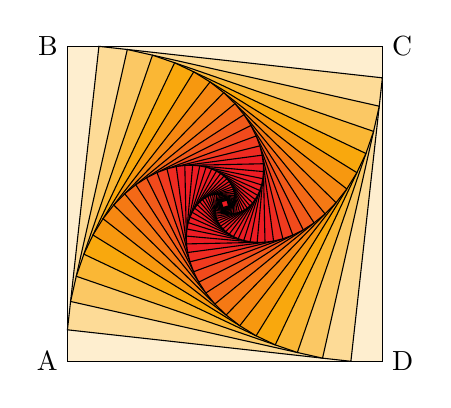
\begin{tikzpicture}
  \newcounter{density}
  \setcounter{density}{20}
  \def\couleur{Dandelion}
  \path[coordinate] (0,0) coordinate(A)
              ++( 90:4cm) coordinate(B)
              ++(0:4cm) coordinate(C)
              ++(-90:4cm) coordinate(D);
  \draw (A) node[left] {A}
    (B) node[left] {B}
    (C) node[right] {C}
    (D) node[right] {D};
  \draw[fill=\couleur!\thedensity] (A)--(B)--(C)--(D)--cycle;
  \foreach \x in {1,...,40}{%
      \pgfmathsetcounter{density}{\thedensity+25}
      \setcounter{density}{\thedensity}
      \path[coordinate] coordinate(X) at (A){};
      \path[coordinate] (A) -- (B) coordinate[pos=.1](A)
                          -- (C) coordinate[pos=.1](B)
                          -- (D) coordinate[pos=.1](C)
                          -- (X) coordinate[pos=.1](D);
      \draw[fill=\couleur!\thedensity] (A)--(B)--(C)--(D)--cycle;
  }
\end{tikzpicture}

  \caption{tikz例子}
  \label{fig:tikzrot}
\end{figure}

\begin{figure}[htb]
  
\includegraphics[width=4cm]{nuaa-logo.pdf}
  \caption{一个校徽}
  \label{fig:logo}
\end{figure}

如果需要多个插图共用一个题注的话,需要加载额外的宏包,
一般选用 \pkg{subcaption} 或 \pkg{subfig},这两个宏包是互斥的。
需要注意的是 \pkg{subcaption} 貌似与 \pkg{geometry} 有些冲突,
会导致多行的图表的最后一行无法居中,而 \pkg{geometry} 是设置页边距的必用宏包。
所以个人推荐使用  \pkg{subfig},效果可以参考\autoref{fig:sub2}。

\begin{figure}[htb]
  \subfloat[左边的大校徽\label{fig:sub1}]{
\includegraphics[width=4cm]{nuaa-logo.pdf}}\quad
  \subfloat[短标题:小校徽][小校徽,题注很长,不过请各位放心,它会自动换行\label{fig:sub2}]
  {
\includegraphics[width=3cm]{nuaa-logo.pdf}}
  \caption{包含两张图片的插图}
  \label{fig:subfigs}
\end{figure}

如果需要插入图表的话,可以考虑使用 \pkg{pgfplots} 宏包,效果参见\autoref{fig:plots};
也可以用 Matplotlib、MatLab、Mathematica 之类的工具导出成兼容格式的图片。

\begin{figure}[htb]
  \subfloat[二维图像\label{fig:func}]{%\documentclass{ctexart}
%\usepackage{pgfplots}
%\pgfplotsset{compat=1.16}
%\begin{document}
\begin{tikzpicture}
  \pgfplotstableread[
    % col sep=comma
  ]{data/plot_2d.csv}{\Data}
  \begin{axis}[
    width=.45\textwidth,
    xmin=0, xmax=16, xtick distance=4,
    xlabel={序列},
    ymin=0, ymax=1,
    ylabel={正确率},
    grid=both,
    legend pos=south east,
  ]
    \addplot+ table[x=idx, y=parray] {\Data};
    \addlegendentry{环境1};
    \addplot+[mark=o] table[x=idx, y=pround] {\Data};
    \addlegendentry{环境2};
  \end{axis}
\end{tikzpicture}
%\end{document}
} \quad
  \subfloat[三维图像\label{fig:sum}]{%\documentclass{minimal}
%\usepackage{pgfplots}
%\pgfplotsset{compat=1.16}
%\begin{document}
\begin{tikzpicture}
  \pgfplotstableread[
    % col sep=comma
  ]{data/plot_3d.csv}{\Data}
  \begin{axis}[
    width=.45\textwidth,
    view={-30}{30},
    xmin=0, xmax=16, xtick distance=4,
    xlabel={Num},
    ymin=1, ymax=20, ytick distance=5,
    ylabel={Round},
    zmin=0, zmax=1, ztick distance=.2,
    zlabel={PDF},
    z tick label style={
      /pgf/number format/.cd,
        fixed,
        fixed zerofill,
        precision=1,
      /tikz/.cd
      },
    grid=major,
  ]
    \addplot3[
      surf,
      mesh/rows=17,
      patch type=rectangle,
      opacity=1,fill opacity=0.1,
      colormap/cool
    ] table[x=num, y=round, z=p] {\Data};
  \end{axis}
\end{tikzpicture}
%\end{document}
}
  \caption{拙作中利用 \pkg{pgfplot} 绘制的图表}
  \label{fig:plots}
\end{figure}

如果真的需要让十几张图片共用一个题注的话,
需要手工拆分成多个 \env{float} 并用 \cs{ContinuedFloat} 来拼接,
不过直接多次使用 \cs{caption} 会在图表清单里产生多个重复条目,需要一点点小技巧
(设置图表目录标题为空)。
建议将浮动位置指定为 \verb|t|,以确保分散至多页的图能占用整个页面,手工分页才能靠谱。
效果可以参见\autoref{fig:subfigss} 的\autoref{fig:logo6}。

\begin{figure}[t]
  \subfloat[校徽$\times 1$]{
\includegraphics[width=4cm]{nuaa-logo.pdf}}\quad
  \subfloat[校徽$\times 2$]{
\includegraphics[width=.4\textwidth]{nuaa-logo.pdf}}\\
  \subfloat[校徽$\times 3$]{
\includegraphics[width=.4\textwidth]{nuaa-logo.pdf}}\quad
  \subfloat[校徽$\times 4$]{
\includegraphics[width=4cm]{nuaa-logo.pdf}}
  \caption{包含多张图片的插图}
  \label{fig:subfigss}
\end{figure}
\begin{figure}[t]
  \ContinuedFloat
  \subfloat[校徽$\times 5$]{
\includegraphics[width=4cm]{nuaa-logo.pdf}}\quad
  \subfloat[校徽$\times 6$ \label{fig:logo6}]{
\includegraphics[width=4cm]{nuaa-logo.pdf}}\\
  \subfloat[校徽$\times 7$]{
\includegraphics[width=4cm]{nuaa-logo.pdf}}\quad
  \subfloat[校徽$\times 8$]{
\includegraphics[width=4cm]{nuaa-logo.pdf}}
  % 指定图表清单中的标题为[],即可将其消除,避免目录中出现重复条目
  \caption[]{包含多张图片的插图(续)}
\end{figure}

如果需要插入一张很大的图片的话,可以使用 \pkg{rotating} 提供的 \env{sidewaysfigure},
它能将插图放置在单独的页面上,如果文档使用 \verb|twoside| 选项的话,它会根据页面方向,
设置 \ang{90} 或 \ang{270} 旋转,可能需要编译两遍才能设置正确的旋转方向。
不过可能有一个问题,\env{sidewaysfigure} 中使用 \cs{subfloat} 可能无法准确标号,
需要手工重置 \texttt{subfigure} 计数器。
效果参见\autoref{fig:fullpage1} 和\autoref{fig:fullpage2}。

\setcounter{subfigure}{0}
\begin{sidewaysfigure}
  \subfloat[First caption\label{fig:fp1}]{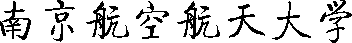
\includegraphics[width=.8\textheight]{nuaa-jianqi.pdf}} \\
  \subfloat[Second caption]{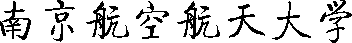
\includegraphics[height=2cm]{nuaa-jianqi.pdf}}
  \caption{一幅占用完整页面的图片}
  \label{fig:fullpage1}
\end{sidewaysfigure}

\setcounter{subfigure}{0}
\begin{sidewaysfigure}
  \subfloat[First caption]{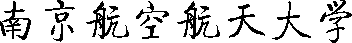
\includegraphics[height=2cm]{nuaa-jianqi.pdf}} \\
  \subfloat[Second caption]{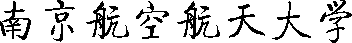
\includegraphics[width=.8\textheight]{nuaa-jianqi.pdf}}
  \caption{又一幅占用完整页面的图片}
  \label{fig:fullpage2}
\end{sidewaysfigure}

\section{表格}

由于封面页,本模板预先加载了 \pkg{array} 和 \pkg{tabu},如果需要其他表格的宏包,
请自行加载。

如果需要插入一个简易的表格,可以只使用 \env{tabular} 环境,如\autoref{tab:city}。
\begin{table}[htb]
  \caption[城市人口]{城市人口数量排名 (source: Wikipedia)\label{tab:city}}
  \begin{tabular}{lr}
    \toprule
    城市 & 人口 \\
    \midrule
    Mexico City & 20,116,842\\
    Shanghai & 19,210,000\\
    Peking & 15,796,450\\
    Istanbul & 14,160,467\\
    \bottomrule
  \end{tabular}
\end{table}

也可以使用 \env{tabu} 环境,它可以更灵活地设置列宽,但它有一些 bug,如\autoref{tab:tabu}。
\begin{table}[htb]
  \caption{\env{tabu} 注意事项 \label{tab:tabu}}
  \begin{tabu} to .9\textwidth {XX[2]<{\strut}} \toprule
    默认列 & 有修正的列 \\ \midrule
    \env{tabu} 的 bug? \par This line is BAD & 注意左侧最后一行后的垂直空格 \\ \midrule
    注意对比最后一行 &
      bug 会影响多行的 \env{tabu} 表格 \par
      bug 的修正方法是在段落后面加 \cs{strut} \par
      This line is Good \\ \midrule
    垂直居中没效果 & 改用 \env{tabular} \\ \midrule
    与新版 \pkg{array} 不兼容 & 谨慎使用,切勿用 \texttt{tabu spread} \\ \bottomrule
  \end{tabu}
\end{table}

如果需要对某一列的小数点对齐,或者带有单位,或者需要做四舍五入的处理,可以尝试配合 \pkg{siunitx} 一起使用。
非常推荐看一下 \pkg{siunitx} 文档的,至少看一下“Hints for using siunitx”一节的输出结果,
\autoref{tab:xmpl:mixed} 来自于该文档的 7.14 节。

\begin{table}[htb]
  \caption{Tables where numbers have different units}
  \label{tab:xmpl:mixed}
  \begin{tabular}
    {
      >{$}l<{$}
      S[table-format = 2.3(1)]
      S[table-format = 3.3(1)]
    }
    \toprule
      & {One} & {Two} \\
    \midrule
    a / \si{\angstrom}   &  1.234(2) &   5.678(4) \\
    \beta / \si{\degree} & 90.34(4)  & 104.45(5)  \\
    \mu / \si{\per\mm}   &  0.532    &   0.894    \\
    \bottomrule
  \end{tabular}
  \hfil
  \begin{tabular}
    {S[table-format=1.3]@{\,}s[table-unit-alignment = left]}
    \toprule
    \multicolumn{2}{c}{Heading} \\
    \midrule
    1.234 & \metre   \\
    0.835 & \candela \\
    4.23  & \joule\per\mole \\
    \bottomrule
  \end{tabular}
\end{table}

如果表格内容很多,导致无法放在一页内的话,需要用 \env{longtable} 或 \env{longtabu} 进行分页。
\autoref{tab:performance} 是来自 \cquthesis{} 的一个长表格的例子。

\begin{longtable}[c]{c*{6}{r}}
	\caption[实验数据]{实验数据,这个题注十分的长,注意这在索引中的处理方式,还有 \cs{caption} 后面的双反斜杠}\label{tab:performance}\\
	\toprule
	\multirow{2}{*}{测试程序} & \multicolumn{1}{c}{正常运行} & \multicolumn{1}{c}{同步} & \multicolumn{1}{c}{检查点} & \multicolumn{1}{c}{卷回恢复}
	& \multicolumn{1}{c}{进程迁移} & \multicolumn{1}{c}{检查点} \\
	& \multicolumn{1}{c}{时间 (s)}& \multicolumn{1}{c}{时间 (s)}&
	\multicolumn{1}{c}{时间 (s)}& \multicolumn{1}{c}{时间 (s)}& \multicolumn{1}{c}{时间 (s)}& \multicolumn{1}{c}{文件 (KB)} \\ \midrule
	\endfirsthead
	\multicolumn{7}{c}{\nuaafontcaption 续表~\thetable\hskip1em 实验数据}\\
	\toprule
	\multirow{2}{*}{测试程序} & \multicolumn{1}{c}{正常运行} & \multicolumn{1}{c}{同步} & \multicolumn{1}{c}{检查点} & \multicolumn{1}{c}{卷回恢复}
	& \multicolumn{1}{c}{进程迁移} & \multicolumn{1}{c}{检查点} \\
	& \multicolumn{1}{c}{时间 (s)}& \multicolumn{1}{c}{时间 (s)}&
	\multicolumn{1}{c}{时间 (s)}& \multicolumn{1}{c}{时间 (s)}& \multicolumn{1}{c}{时间 (s)}& \multicolumn{1}{c}{文件(KB)} \\ \midrule
	\endhead
	\hline
	\multicolumn{7}{r}{续下页}
	\endfoot
	\endlastfoot
	CG.A.2 & 23.05 & 0.002 & 0.116 & 0.035 & 0.589 & 32491 \\
	CG.A.4 & 15.06 & 0.003 & 0.067 & 0.021 & 0.351 & 18211 \\
	CG.A.8 & 13.38 & 0.004 & 0.072 & 0.023 & 0.210 & 9890 \\
	CG.B.2 & 867.45 & 0.002 & 0.864 & 0.232 & 3.256 & 228562 \\
	CG.B.4 & 501.61 & 0.003 & 0.438 & 0.136 & 2.075 & 123862 \\
	CG.B.8 & 384.65 & 0.004 & 0.457 & 0.108 & 1.235 & 63777 \\
	MG.A.2 & 112.27 & 0.002 & 0.846 & 0.237 & 3.930 & 236473 \\
	MG.A.4 & 59.84 & 0.003 & 0.442 & 0.128 & 2.070 & 123875 \\
	MG.A.8 & 31.38 & 0.003 & 0.476 & 0.114 & 1.041 & 60627 \\
	MG.B.2 & 526.28 & 0.002 & 0.821 & 0.238 & 4.176 & 236635 \\
	MG.B.4 & 280.11 & 0.003 & 0.432 & 0.130 & 1.706 & 123793 \\
	MG.B.8 & 148.29 & 0.003 & 0.442 & 0.116 & 0.893 & 60600 \\
	LU.A.2 & 2116.54 & 0.002 & 0.110 & 0.030 & 0.532 & 28754 \\
	LU.A.4 & 1102.50 & 0.002 & 0.069 & 0.017 & 0.255 & 14915 \\
	LU.A.8 & 574.47 & 0.003 & 0.067 & 0.016 & 0.192 & 8655 \\
	LU.B.2 & 9712.87 & 0.002 & 0.357 & 0.104 & 1.734 & 101975 \\
	LU.B.4 & 4757.80 & 0.003 & 0.190 & 0.056 & 0.808 & 53522 \\
	LU.B.8 & 2444.05 & 0.004 & 0.222 & 0.057 & 0.548 & 30134 \\
	CG.B.2 & 867.45 & 0.002 & 0.864 & 0.232 & 3.256 & 228562 \\
	CG.B.4 & 501.61 & 0.003 & 0.438 & 0.136 & 2.075 & 123862 \\
	CG.B.8 & 384.65 & 0.004 & 0.457 & 0.108 & 1.235 & 63777 \\
	MG.A.2 & 112.27 & 0.002 & 0.846 & 0.237 & 3.930 & 236473 \\
	MG.A.4 & 59.84 & 0.003 & 0.442 & 0.128 & 2.070 & 123875 \\
	MG.A.8 & 31.38 & 0.003 & 0.476 & 0.114 & 1.041 & 60627 \\
	MG.B.2 & 526.28 & 0.002 & 0.821 & 0.238 & 4.176 & 236635 \\
	MG.B.4 & 280.11 & 0.003 & 0.432 & 0.130 & 1.706 & 123793 \\
	MG.B.8 & 148.29 & 0.003 & 0.442 & 0.116 & 0.893 & 60600 \\
	LU.A.2 & 2116.54 & 0.002 & 0.110 & 0.030 & 0.532 & 28754 \\
	LU.A.4 & 1102.50 & 0.002 & 0.069 & 0.017 & 0.255 & 14915 \\
	LU.A.8 & 574.47 & 0.003 & 0.067 & 0.016 & 0.192 & 8655 \\
	LU.B.2 & 9712.87 & 0.002 & 0.357 & 0.104 & 1.734 & 101975 \\
	LU.B.4 & 4757.80 & 0.003 & 0.190 & 0.056 & 0.808 & 53522 \\
	LU.B.8 & 2444.05 & 0.004 & 0.222 & 0.057 & 0.548 & 30134 \\
	EP.A.2 & 123.81 & 0.002 & 0.010 & 0.003 & 0.074 & 1834 \\
	EP.A.4 & 61.92 & 0.003 & 0.011 & 0.004 & 0.073 & 1743 \\
	EP.A.8 & 31.06 & 0.004 & 0.017 & 0.005 & 0.073 & 1661 \\
	EP.B.2 & 495.49 & 0.001 & 0.009 & 0.003 & 0.196 & 2011 \\
	EP.B.4 & 247.69 & 0.002 & 0.012 & 0.004 & 0.122 & 1663 \\
	EP.B.8 & 126.74 & 0.003 & 0.017 & 0.005 & 0.083 & 1656 \\
	\bottomrule
\end{longtable}

\section{数字与国际单位}

本模板预加载 \pkg{siunitx} 来格式化文中的内联数字,该宏包有大量可定制的参数,
请务必阅读其文档,并在文档导言部分设置格式。

\begin{itemize}
  \item 旋转角度为 \ang{90}、\ang{270}
  \item 分辨率 \num{1920x1080} 的像素数量约为 \num{2.07e6}
  \item 电脑显示器的像素间距为 \SI{1.8}{\nm}、\SI{180}{\um} 还是 \SI{18}{\mm}?
  \item 重力加速度 $g=\SI{9.8}{\kg\per\square\second}$、
  $g=\SI[inter-unit-product=\ensuremath{{}\cdot{}}]{9.8}{\kg\per\square\second}$,
  亦或 $g=\SI[per-mode=symbol]{9.8}{\kg\per\square\second}$
\end{itemize}

\section{中英文之间空格}

很遗憾,目前 \LaTeX{} 和 \CTeX{} 虽然能处理普通汉字与英文之间的间隔,
但是汉字与宏之间的空格仍然需要手工调整,请务必按以下的规则撰写原稿:
\begin{itemize}
  \item[\ding{51}] 如\autoref{fig:sub2} 所示:\verb|如\autoref{fig:sub2} 所示|,这个宏返回的是“图 x.xx”,
  所以前面两个汉字之间不能加空格,后面数字与汉字之间必须加空格;
  \item[\ding{51}] 距离为 1.7~个天文单位:\verb|距离为 1.7~个天文单位|,前面可以不加空格(\CTeX 会修正),
  后面必须加 \verb|~| 以防止在 “1.7”与“个”之间换行。此时更推荐写成 \SI{1.7}{au}:\verb|\SI{1.7}{au}|。
\end{itemize}


\appendix
% 如果需要附录的话,在这里 include
\chapter{查重和其他注意事项}

本节由 Old Jack 写于 2017年六月\footnote{\url{https://github.com/nuaatug/nuaathesis/commit/1155207}}。

\section{查重}

先说结论:{\large\textbf{知网完全支持pdf查重}}。

这个问题是鄙人整个毕设过程中最担心的问题之一,从知乎以及其他各种渠道搜索的结果并不一致;另外关于pdf查重具体检测哪些部分也是有很多种说法,现在根据鄙人论文的检测结果来说明一下几个需要注意的地方:

\begin{itemize}
  \item \textbf{页眉页脚:} pdf的眉页脚在论文查重检测范围内。如果担心会提升重复率,可以将页眉文字去掉(个人认为没必要);
  \item \textbf{公式环境:} pdf中的公式在论文查重检测范围内。所以在编辑公式的时候,可以考虑不使用传统符号来编辑公式(物理公式符号不建议使用这种方法,各物理量的符号比较固定,老师可能会要求改正),以降低重复率,如参考文献中使用$\alpha$,可以改为$a$或$x$诸如此类;
  \item \textbf{表格环境:} 鄙人的论文中没有直接证据,但根据公式环境在查重检测范围内,鄙人推断表格的标题和内容很有可能也在范围内,所以建议大家不要直接摘抄实验数据和表格标题;
  \item \textbf{参考文献:} 鄙人在使用淘宝知网论文检测时,并未提交参考文献部分,学校不提供论文检测结果,所以目前没有直接证据证实参考文献是否在查重范围之内;
  \item \textbf{附录:} 鄙人的论文没有附录,情况不明。
\end{itemize}

鄙人的老师开始也要求上交word版论文,但是在鄙人的坚持下,最终上交了pdf版并成功通过查重。建议大家提前和指导老师打好招呼,最后提交pdf格式的论文。

\section{批注}
在论文撰写过程中,批注成了一个问题,鄙人的指导学姐并不是计算机专业出身,对\LaTeX 和基于Git的版本管理并不了解,所以沟通的途径就只有使用Adobe Acrobat等软件,对pdf文件本身进行批注,相比于word确实有些麻烦。

个人还是推荐使用Git\footnote{\url{https://git-scm.com/}}、Beyond Compare\footnote{\url{https://www.scootersoftware.com/}}等工具,辅以\LaTeX 本身的注释进行批注以及版本管理,非常清晰直观,操作也简单。

\section{毕业设计与毕业论文的区别}
这里特别对使用本模板的本科同学们做出提醒,请查看你们毕业设计基本信息中的毕设类别,共有两类:\textbf{毕业设计}和\textbf{毕业论文}。各位同学,你们\textbf{论文的封面和页眉中的内容应该与该类别相同}。因此在\verb!\documentclass[]{nuaathesis}!的选项中需要标明\textbf{Design}(毕业设计)或者\textbf{Paper}(毕业论文),使论文使用正确的封面和页眉。

除此之外该两类在最后论文装订时使用的并不是同一种封面纸,\textbf{毕业设计类的论文使用黄色的封面,毕业论文类的论文使用白色的封面}。在印刷厂/打印店打印时需提醒工作人员使用正确的封面纸张。

\section{单面打印\& 双面打印}
学校并没有规定论文打印的方式,考虑到部分同学有双面打印的需求,Gavin Lee 对twoside情况下的页脚进行了调整,奇数页页脚在右边,偶数页页脚在左边。可以在文档选项中使用oneside/twoside来切换单面打印和双面打印。

\section{封面打印\& 装订}
建议大家去印刷厂打印封面并装订。原因有下:
\begin{enumerate}
  \item 樱花广场打印店打印的封面并不标准,情况较复杂,总之是不标准的;
  \item 樱花广场打印店打印机并不稳定可靠,而且因为所有电脑都可以随意选择打印机,所以很容易出现打印错误,鄙人曾因员工操作失误以及机器故障被耽误2小时;
  \item 樱花广场打印店的档案袋储量较小,可能会用尽,而印刷厂不单独出售毕设档案袋,只能额外花钱买一整套封面来获取档案袋,存在浪费钱财的可能;
  \item 樱花广场打印店排队情况严重,因为有很多同学会在那里的电脑上修改他们的文档,从而影响了打印的效率。
\end{enumerate}

印刷厂虽远,但其质量是有保证的,封面也是标准的,另外因为距离远,排队现象相对较好,所以鄙人建议大家去印刷厂打印封面。

在印刷厂打印需要事先打好三个\textbf{A4纸}封面(论文封面、附件材料封面、工作材料归档封面),然后会使用你打印好的A4纸封面,复印到封面纸上,就得到了你的封面。

\chapter{后记}

\section{v0.9a后记——Old Jack 的吐槽}

\verb!\begin{轻松+愉快}!

Old Jack 他有点累......

Old Jack 两年前就开始关注南航毕设的\LaTeX 模板了,但是两年了还没有任何有实际意义的新动作,所以Old Jack 就亲自操刀制作了新的一版。虽然很多代码都是从其他模板中直接摘抄过来的,但是这也是\TeX 最普遍、最快捷的学习\&开发方法。一开始 Old Jack 也想造轮子,但是轮子真的不好造。

在制作过程中遇到了几个关键性的问题:
\begin{itemize}
  \item 前文提到的三种粗体
  \item nuaa.png源文件和页眉制作
  \item 英文字母、章节标题莫名其妙的加粗
  \item 脚注相对页脚线的位置
\end{itemize}

第一个问题 Old Jack 曾经用\TeX 中伪粗体(FakeBold)的方法实现过,但是效果并不好,而且当时受到最后一个问题的强烈影响,不得不使用其他字体来解决这个问题。

第二个问题 Old Jack 开始是使用官方模板中的图片,但是分辨率太低,效果很差。于是 Old Jack Google以图搜图找到了现在的这个文件的源文件,经过了一系列不可描述的操作后得到了现在的 nuaa.png 。页眉的制作也让 Old Jack 很头疼,论文要求论文到顶端和底端的距离分别为2.5cm和2.0cm,Old Jack 很naive的就给geometry设置了这个数值,但是效果和官方模板差了很多,于是 Old Jack 只好一点一点地调试,达到了近似官方模板的效果。页脚和官方模板有细微的区别,Old Jack 认为这无伤大雅,是要罗马数字和阿拉伯数字编号正确应该就可以了。

第三个问题是一个非常奇怪的问题。使用伪粗体时所有标题全都加粗了,非常难看,经过了代码重构和不停地调试解决了这个问题。在模板完成99\% 后发现最后致谢中的英文字体全都加粗了, Old Jack 几次审视代码和调试都没有解决。偶然间,Old Jack 将全部主要文件全部提取出来,放入另一个文件夹,然后重新编译就解决了这个问题!当然后来发现代码中确实有一个地方有小问题\textbf{可能}会影响,但是这不是上一次出错的原因。Old Jack 对于各位使用模板的南航学子以及其他可能会参考此模板的\TeX 爱好者提了一个建议:\textbf{任何语言,任何代码出现莫名其妙的问题时,换一个文件夹,改一下名字,重新跑一下,可能会得到意想不到的结果。}当然这不是万能的解决方法。

第四个问题就如第一章中脚注和页脚线的情况,感觉两条线很别扭。 Old Jack 犹豫了很久,最后没有采用将脚注放在页脚线下的方案,因为 Old Jack 觉得还是两条线的方案好看。对于想要将脚注放在页脚线下方的同学,可以在主文件中取消注释那段代码,来实现所需要的效果。

Old Jack 他完成了模板的再制作,但是他没有心气再写出一篇能够指导大家使用\LaTeX 的文档了(好吧,Old Jack 他承认懒是一部分因素),望大家谅解 Old Jack。

\verb!\end{轻松+愉快}!

\section{v1.0后记}

Old Jack 非常高兴,因为他不是一个人在战斗。再次感谢张一白、王成欣、曾宪文、Gavin Lee等人的工作,没有他们,\nuaathesis 不会像现在这么美丽。

经过\nuaathesis~Group的努力和测试,\nuaathesis 迎来了v1.0版,也就是第一个正式发行版。一路走来也是有些坎坷,各种各样的小问题一直困扰着我们,其实v1.0 也还有着一些细小的问题尚未解决。不过Old Jack请大家放心,这些小问题不影响模板的使用。很多已经被我们解决的小问题比如页眉的大小位置,中英文字体是否正确,摘要的章节标题不能是加粗的宋体等等,老师可能不去管这些,甚至注意不到有什么区别。相比之下,重要的地方是:公式、图表的编号,图表和文本的位置,参考文献的格式等等才是老师关注的点。很多地方只是我们几个人为了追求和office模板尽可能接近,才不断地进行修改调整,也是有点讽刺。

写毕设论文的时候,Old Jack 不止一次看到隔壁室友调公式内容,Mathtype和Office装了卸,卸了装、调公式编号、调标题位置和大小、调首行缩进、调段间距等等等等,看着他们搞得焦头烂额的,Old Jack 都觉得心累。打印时也是这样,有太多的人在打印店不停地修改自己的论文,有因为office和wps不兼容修改的,有office版本不兼容修改的,有因为页眉页脚错误修改的等等。然而 Old Jack 他在写论文时从来没有担心过这些事情(当然,作为模板开发者 Old Jack 确实操心了很多,2333),他也第一次真正体会到了什么叫做专注于内容,真的挺轻松的(表格是例外)。

对于模板的推广,Old Jack觉得使用人数仍然不会太多,毕竟\LaTeX 的群众基础太小,除了8院,其他学院对公式的需求整体来讲并不迫切,Old Jack 猜测大部分知道、了解\LaTeX 的同学是通过数学建模竞赛这个途径才学习了\LaTeX ;同时因为涉及到学习新的程序语言,时间成本也较大,所以很多同学的学习意愿不高。不过\nuaathesis 的目标人群本来也不是全校所有学生,Old Jack 的思路,Old Jack 相信也是\nuaathesis~Group其他开发者的思路是:
\begin{enumerate}
  \item 为自己服务,这是\nuaathesis~Group开发模板的第一动力;
  \item 对已经掌握\LaTeX 基本语法的同学,\nuaathesis~Group为他们在毕业设计时能更轻松地撰写论文,提供平台和机会;
  \item 对准备学习\LaTeX 以及已经学习了一点\LaTeX 的同学,\nuaathesis~Group为他们提供学下去的动力和平台。
\end{enumerate}

即将毕业了,回首大学四年, Old Jack 做过疯狂的事情,也找到了一份看起来还可以的工作,只觉得还没对学校做过什么有用的事情,尽管 Old Jack 对学校其实并不是很有感情。完成了这个模板后,至少 Old Jack 可以减少一个遗憾,然后离开学校了。虽然这不是什么惊天动地的工作,但是至少 Old Jack 做了件他认为还算有意义的事情。Old Jack应该还会再维护\nuaathesis 一段时间,期待有后继者能够接过火炬,继续完善并推广\nuaathesis 。

想说的可能也就这么多了,Old Jack out!

\hfill 0813~王志浩,2017.6.24

\section{v2.0 后记 by yzwduck}

也是两年前开始关注南航毕设的\LaTeX 模板了,但直到毕业前,都没能去静下心来学习\LaTeX。

现在差不多本科毕业一年,或者说,一年后要开写硕士学位论文了,
本打算照着 CQUThesis 来造轮子的时候,逛纸飞机\footnote{论坛还活着吗?该不会已经沦落为老人的回忆了吧。 ——2018.10.10}
看到 \nuaathesis~v1.0 发布了。
非常激动、也很自愧,同样是经历了大学四年的人,我没能把这模板做出来。

于是马上把两年前为了模板而画的校名(矢量图)传了上去\footnote{\url{https://github.com/nuaatug/nuaathesis/commit/24fa82e}}。

原本打算在 v1.0 版的基础上修改的,但因为行间距设置有问题,封面与 Word 模板也有点差异,
还要再加入硕/博士的模板,于是干脆改成 \texttt{Documented LaTeX Source (.dtx)},
方便以后写模板的文档。

做模板过程中遇到的大问题,在于如何正确理解学校对论文格式的要求。
虽然有《本科毕业设计(论文)撰写格式要求》、《研究生学位论文撰写要求》,
但这些要求依然不够细致,因为那些要求都是假定你用 Word 来写论文的,要求里的内容是 Word 设置的操作方法,
所以还要先学习 Word 的排版算法。虽然这不是热门的资料,而且还有 CJK 独有的坑,
幸好有人把 Word 排版算法解释得非常详细,这个模板才能避免大量使用测量得到的魔数。
但还有很多细节部分,因为能力有限,没能实现。

最后容我吐槽一下学校的 Word 模板,我觉得那个 Word 模板可能从最初做出来后,就基本没有变化。
那个“最初”或许可以追溯到上个世纪。很多编号的事情都要由手工来完成,比如说目录页码、
各级标题的编号、题注等。这些完全可以自动编号的工作,如果要手工做的话【掀桌颜文字】。

\section{v2.1 后记 by yzwduck}

转眼间一年过去,又到了写毕业论文的时候了。

翻了一下代码的 commit 记录(部分非公开),这一年间只有加起来两、三个星期在做这个论文模板,
已经无法用“懒”这字来描述鄙人的状态了。

不过也有几件值得小小炫耀一下的事,终于把中/英/日多国语的坑填了不少,至少能编译出对应语言的论文来;
为了减少重复代码,使用一些宏包造了 \CTeX{} 的几个轮子,从而实现一个 class 文件能支持三国语言。

为了检验模板的效果,鄙人从知网上找了两篇论文,试着用 \nuaathesis{} 模板排版了一下(节选),又发现了不少问题。
因此目前 \nuaathesis{} 应该还有相当多的问题的,但没有用户的话,由于鄙人能力有限,难以发现,
还请各位使用 \nuaathesis{} 的先行者们(Pioneers) 能反馈意见和建议。

愿所有使用 \nuaathesis{} 的人,不会被评审老师指责格式问题。


\backmatter
% 如果参考文献使用 biber
\bibliographystyle{nuaabib}   % 参考文献的样式
\bibliography{bib/sample}   % 参考文献,即 bib/sample.bib 文件(纯文本)
% 如果打算手写参考文献
\chapter{\bibname}

\begin{manref}
\item \label{ref:hint} 手作りの参考文献
\item \zhcn{如果能使用 biber,就不要手写参考文献}
\item \zhcn{如果一定要手写的话,就按照学校的参考文献格式来写,如:}
\item \label{ref:man} KANAMORI H. Shaking without quaking[J]. Science, 1998, 279(5359): 2063.
\end{manref}

例:[\ref{ref:hint}]はヒントです、\mcite{ref:man}は1998年に発表されました。


\chapter[致谢]{致\hskip\ccwd{}谢}

在此感谢对本论文作成有所帮助的人。


\end{document}
